\documentclass[border=1.5pt]{standalone}
\usepackage{amsmath,amssymb}
\usepackage{tikz}
\usetikzlibrary{arrows.meta,calc,positioning,shapes,shapes.misc,shapes.geometric,backgrounds,fit,decorations.pathreplacing,quantikz2}
% Shared colors and styles for the XYZ^2 figures.
% Pauli types: bright tones for fills and bands, deep (800) shades of the same hues for labels.
% The label shades keep the hue of each Pauli, are well separated from each other (CIEDE2000 > 20)
% and have a contrast ratio of at least 2.9 on the coral cells and 4.5 on the sunflower cells.
\definecolor{PauliX}{HTML}{F97316}
\definecolor{PauliY}{HTML}{EC4899}
\definecolor{PauliZ}{HTML}{9333EA}
\definecolor{PauliXText}{HTML}{AC340B}
\definecolor{PauliYText}{HTML}{9D174D}
\definecolor{PauliZText}{HTML}{5B21B6}
% Generator classes: S0 (class B, even links, coral) and gauge (class A, odd links, sunflower)
\definecolor{Szero}{HTML}{F0435E}
\definecolor{SzeroText}{HTML}{BE123C}
\definecolor{Gauge}{HTML}{F59E0B}
\definecolor{GaugeText}{HTML}{B45309}
\colorlet{GaugeGray}{Gauge}
\definecolor{ClassB}{HTML}{FF8A99}
\definecolor{ClassA}{HTML}{FFD23F}
% Logical operators (X-bar violet, Z-bar crimson), errors, ink
\definecolor{LogicalZ}{HTML}{E11D48}
\definecolor{LogicalGold}{HTML}{7C3AED}
\definecolor{ErrRed}{HTML}{1C1917}
\definecolor{InkDark}{HTML}{292524}
\definecolor{InkSoft}{HTML}{57534E}
% Labels drawn on top of colored cells
\colorlet{CellText}{InkDark}
% Noise channels
\definecolor{ErrFlip}{HTML}{EF4444}
\definecolor{Idle}{HTML}{EC4899}
\definecolor{TwoQ}{HTML}{7C3AED}
% Protocol steps
\definecolor{StepPrep}{HTML}{F97316}
\definecolor{StepMeas}{HTML}{D946EF}
\definecolor{StepDec}{HTML}{7C3AED}
\definecolor{StepRec}{HTML}{DB2777}
\tikzset{
  qb/.style={circle, draw=InkDark, line width=0.6pt, fill=white,
             minimum size=4.2mm, inner sep=0pt, font=\scriptsize},
  qbsmall/.style={circle, draw=InkDark, line width=0.5pt, fill=white,
             minimum size=2.6mm, inner sep=0pt},
  hexedge/.style={line width=0.65pt, draw=InkSoft},
  linkedge/.style={line width=1.6pt, draw=InkDark},
  bndedge/.style={line width=0.65pt, draw=InkSoft, densely dashed},
  plabel/.style={font=\scriptsize\bfseries, inner sep=1pt},
  panel/.style={font=\small\bfseries, anchor=north west},
}

\providecommand{\ket}[1]{\left|#1\right\rangle}

\begin{document}
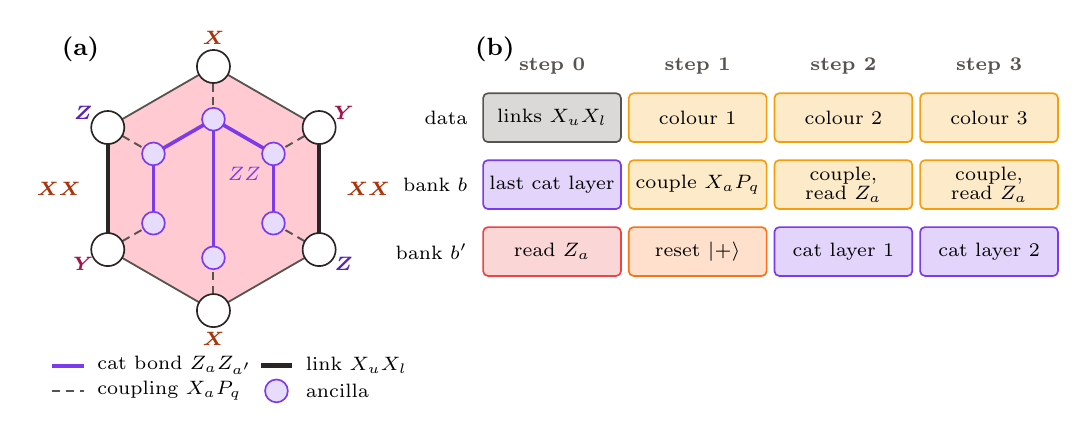
\begin{tikzpicture}[
  anc/.style={circle, draw=TwoQ, line width=0.6pt, fill=TwoQ!18, minimum size=2.9mm, inner sep=0pt},
  zz/.style={line width=1.3pt, draw=TwoQ},
  cpl/.style={line width=0.7pt, draw=InkSoft, densely dashed},
  step/.style={draw=#1, fill=#1!22, line width=0.6pt, rounded corners=0.6mm, minimum height=0.62cm, minimum width=1.75cm, text width=1.62cm, font=\scriptsize, inner sep=1pt, align=center},
]
% ---------------------------------------------------------------- (a) one hexagon
\node[panel] at (-2.05,2.05) {(a)};
\def\R{1.55}
\def\r{0.88}
% data qubits: angle, name, Pauli, label side
\foreach \a/\n/\p in {90/t/X, 150/blu/Z, 210/bll/Y, 270/b/X, 330/trl/Z, 30/tru/Y}{
  \coordinate (D\n) at (\a:\R);
  \coordinate (A\n) at (\a:\r);
}
\fill[ClassB!45] (90:\R) -- (150:\R) -- (210:\R) -- (270:\R) -- (330:\R) -- (30:\R) -- cycle;
\draw[hexedge] (90:\R) -- (150:\R) (210:\R) -- (270:\R) -- (330:\R) (30:\R) -- (90:\R);
% links: the two vertical edges, measured directly
\draw[linkedge] (Dblu) -- (Dbll);
\draw[linkedge] (Dtru) -- (Dtrl);
\node[font=\scriptsize, text=InkDark, anchor=east] at ($(Dblu)!0.5!(Dbll)+(-0.22,0)$) {$\textcolor{PauliXText}{\boldsymbol{X}}\textcolor{PauliXText}{\boldsymbol{X}}$};
\node[font=\scriptsize, text=InkDark, anchor=west] at ($(Dtru)!0.5!(Dtrl)+(0.22,0)$) {$\textcolor{PauliXText}{\boldsymbol{X}}\textcolor{PauliXText}{\boldsymbol{X}}$};
% couplings X_a P_q
\foreach \n in {t, blu, bll, b, trl, tru}{ \draw[cpl] (A\n) -- (D\n); }
% cat tree: centre at the top ancilla
\draw[zz] (At) -- (Ablu);
\draw[zz] (Ablu) -- (Abll);
\draw[zz] (At) -- (Atru);
\draw[zz] (Atru) -- (Atrl);
\draw[zz] (At) -- (Ab);
\foreach \n in {t, blu, bll, b, trl, tru}{ \node[anc] at (A\n) {}; }
\foreach \a/\n/\p in {90/t/X, 150/blu/Z, 210/bll/Y, 270/b/X, 330/trl/Z, 30/tru/Y}{
  \node[qb] at (D\n) {};
  \node[plabel, text=Pauli\p Text] at (\a:\R+0.36) {$\boldsymbol{\p}$};
}
\node[font=\scriptsize, text=TwoQ, anchor=west] at ($(At)!0.5!(Ab)+(0.06,0.18)$) {$ZZ$};
% legend
\begin{scope}[shift={(-2.05,-2.25)}]
  \draw[zz] (0,0) -- (0.4,0); \node[font=\scriptsize, anchor=west] at (0.45,0) {cat bond $Z_aZ_{a'}$};
  \draw[cpl] (0,-0.32) -- (0.4,-0.32); \node[font=\scriptsize, anchor=west] at (0.45,-0.32) {coupling $X_aP_q$};
  \draw[linkedge] (2.65,0) -- (3.05,0); \node[font=\scriptsize, anchor=west] at (3.1,0) {link $X_uX_l$};
  \node[anc] at (2.85,-0.32) {}; \node[font=\scriptsize, anchor=west] at (3.1,-0.32) {ancilla};
\end{scope}
% ---------------------------------------------------------------- (b) one round
\begin{scope}[shift={(3.35,0)}]
\node[panel] at (-0.15,2.05) {(b)};
\foreach \x/\t in {0.95/step 0, 2.8/step 1, 4.65/step 2, 6.5/step 3}{
  \node[font=\scriptsize\bfseries, text=InkSoft] at (\x,1.55) {\t};
}
\node[font=\scriptsize, anchor=east] at (0.0,0.9) {data};
\node[font=\scriptsize, anchor=east, align=right] at (0.0,0.05) {bank $b$};
\node[font=\scriptsize, anchor=east, align=right] at (0.0,-0.8) {bank $b'$};
\node[step=InkSoft] at (0.95,0.9) {links $X_uX_l$};
\node[step=Gauge] at (2.8,0.9) {colour 1};
\node[step=Gauge] at (4.65,0.9) {colour 2};
\node[step=Gauge] at (6.5,0.9) {colour 3};
\node[step=TwoQ] at (0.95,0.05) {last cat layer};
\node[step=Gauge] at (2.8,0.05) {couple $X_aP_q$};
\node[step=Gauge] at (4.65,0.05) {couple,\\[-1pt] read $Z_a$};
\node[step=Gauge] at (6.5,0.05) {couple,\\[-1pt] read $Z_a$};
\node[step=ErrFlip] at (0.95,-0.8) {read $Z_a$};
\node[step=StepPrep] at (2.8,-0.8) {reset $\ket{+}$};
\node[step=TwoQ] at (4.65,-0.8) {cat layer 1};
\node[step=TwoQ] at (6.5,-0.8) {cat layer 2};
\end{scope}
\end{tikzpicture}

\end{document}
